% the first part of the document before the begin is called preamble
\documentclass[12pt, a4paper]{article}
\usepackage{graphicx}
\graphicspath{ {./images/} }
%
\author{Leonardo Valente}
\title{Basi di Dati}

\begin{document}
    \maketitle
    \tableofcontents
    \section{Modello ER}
    Qualsiasi progetto, prima di essere mandato in produzione, segue un ciclo di vita, di solito composto da:

    \begin{itemize}
        \item Studio di fattibilità: definizione dei costi e delle priorità
        \item Raccolta di analisi e dei requisiti: studio delle proprietà del sistema
        \item Progettazione: di dati e funzioni
        \item Implementazione: ovvero la realizzazzione del progetto
        \item Validazione e collaudio: la fase di sperimentazione
        \item Funzionamento: fase di produzione
        \item Manutenzione: dove arriva il vero guadagno
    \end{itemize}

    Questo ciclo di vita segue un \textbf{modello a spirale}, quindi un ciclo dove in ogni fase è possibile
    andare avanti o indietro in base alle esigenze.

    \subsection{Progettazione}
    La progettazione delle applicazioni schematizza le operazioni sui dati e progetta il software.
    E' opportuno quindi seguire una \textbf{metodologia di progetto}.
    Essa ci permette di \textbf{suddividere} la progettazione in fasi indipenti,
    fornendo delle \textbf{strategie} da seguire e dei \textbf{criteri} di scelta.
    \\
    Nella progettazione di Database ci sono 3 fasi di progettazione: 
    \begin{itemize}
        \item Progettazione concettuale (modello ER)
        \item Progettazione logica
        \item Progettazione fisica
    \end{itemize}
    Ognuna di queste fasi si basa su un modello che permette di generare una rappresentazione
    formale (di solito uno schema) del nostro universo.
    
    \subsubsection{Progettazione concettuale}
    Traduce i requisiti del sistema in un modello ER, espresso in modo indipendente dalle scelte implementative.
    \\La descrizione si deve concentrare sui \textbf{dati} e sulle loro \textbf{relazioni}, non sulle scelte implementative.

    \subsubsection{Progettazione logica}
    Consiste nella traduzione dello schema concettuale nel modello dei dati del DBMS (Modello relazionale).

    \subsubsection{Progettazione fisica}
    Completa lo schema logico ottenuto con le specifiche proprio dell'HW/SW scelto. 
    Viene interamente effettuato dal DBMS. 
    \newpage
    \subsection{Introduzione al Modello ER}
    Il modello Entità - Relazione è un \textbf{linguaggio grafico semi-formale} per la rappresentazione di schemi concettuali.
    Esso è ormai diventato uno \textit{standard} nelle metodologie di progetto.

    Iniziamo facendo una distinzione fra \textbf{Entità} e \textbf{Relazioni}.

    \begin{itemize}
        \item \textbf{Entità}: classe di oggetti dell'applicazione di interesse con proprietà comuni e con esistenza "autonoma",
        della quale si vogliono registrare fatti specifici.
        \\Le entità hanno degli attributi che la descrivono.
        \\Una \textbf{occorrenza} (o istanza) di una entità è il singolo oggetto creato sulla base dell'entità da cui deriva
        \\Le entità vengono rappresentate nel modello ER tramite dei \textit{rettangoli}.
        \item \textbf{Attributi}: un attributo è definito su un dominio di valori.
        Esso è una funzione che associa ad ogni occorrenza \textbf{un} particolare valore (non di più!)
        Gli attributi possono essere composti e possono essere \textbf{qualsiasi cosa}.
        \\A meno che non venga definito il contrario, gli attributi sono \textbf{obbligatori}.
        \item \textbf{Relazione}: fatto che descrive un'azione o una situazione e che \textit{stabilisce legami logici tra istanze di entità}.
        \\I legami possono essere fra più di due entità e il numero delle entià coinvolte ne determina il \textbf{grado}.
        \\Ogni relazione ha un nome che la identifica.
        \\Inoltre, le relazioni possono avere degli attributi, chiamati appunto \textbf{attributi delle relazioni} che
        modellano il legame tra le entità.
        \\\\Le relazioni vengono rappresentate nel modello ER tramite dei \textit{rombi}.
        
    \end{itemize}

    \newpage
    \subsection*{Associazioni ad anello}
    Un'associazione può coinvolgere "due o più volte" la stessa entità (associazione ricorisiva o ad anello).
    \begin{figure}[htbp]
        \centering
        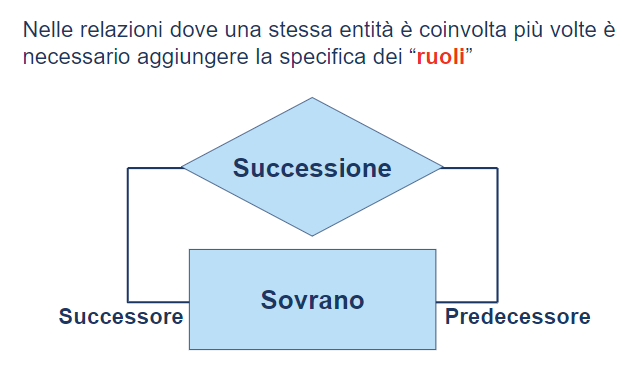
\includegraphics[scale=0.7]{roles.png}
    \end{figure}

    \section{Cardinalità delle Relazioni}
    La cardinalità delle relazioni non è altro che una coppia di valori che si associa
    a ogni entità che partecipa ad una relazione. 
    Esprimono un \textbf{limite minimo} (cardinalità minima) e un \textbf{limite massimo}
    (cardinalità massima) di istanze della \textbf{relazione R} a cui può partecipare ogni
    istanza dell'\textbf{entità E}.
    \\
    E' molto importante non sbagliare la \textit{cardinalità massima}. E' la più importante fra le due.
    Se sbagliamo la cardinalità, sbagliamo il Database!
    \\\\
    \textbf{Nota}: anche gli attributi possono avere cardinalità!
    \begin{itemize}
        \item \textbf{Molti a Molti} (3 tabelle). Quando zero o più istanze della prima entità si possono associare a zero o più istanze della seconda entità.
        \item \textbf{Uno a Molti} (2 tabelle). Quando ogni istanza della prima entità si può associare a una o più istanze della seconda entià.
        \item \textbf{Uno a Uno} (2 tabelle). Quando ogni istanza della prima entità si può associare a una e una sola istanza della seconda entià.
    \end{itemize}
    \newpage
    \subsection{Identificatori di una entità}
    E' uno strumento per l'identificazione univoca delle occorrenze di una entità.
    Ci sono due tipi di identificatori:
    \\\textbf{(!!!! CAMBIARE LE DEFINZIONI NON SONO CORRETTE !!!)}
    \begin{itemize}
        \item \textbf{Identificatore interno} (Primary Key), che serve per distinguere in modo univoco una istanza di una entità.
        \textit{Deve essere unico}.
        \\L'identificatore interno può essere combinazione di più attributi!
        \item \textbf{Identificatore esterno} (Foreign Key), che serve per fare riferimento ad una istanza di un'altra entità avente come
        identificatore primario l'identificatore esterno dell'oggetto che stiamo prendendo in considerazione.
    \end{itemize}
    Ogni entità deve possedere almeno un identificatore (primario), ma può averne in generale più di uno (esterno).

    \section{Relazione IS-A}
    Può accadere che tra due classi rappresentate da due entità nello schema concettuale sussista la 
    \textbf{relazione IS-A}, cioè che \textbf{ogni istanza di una sia anche istanza dell'altra}.
    \\La relazione IS-A si può definire tra \textit{due entità}: \textbf{entità padre} e \textbf{entità figlio}.

    \newpage
    \subsubsection{Generalizzazione}
    Può capitare però, che l'entità padre può generalizzare diverse sottoentità rispetto ad un unico criterio. 
    In questo caso si parla di \textbf{generalizzazione}.
    \\Una generalizzazione può essere di \textit{due tipi}:
    \begin{itemize}
        \item \textbf{Completa}: l'unione delle istanze delle sottoentità è uguale all'insieme delle istanze dell'entità padre.
        \item \textbf{Non completa}.
    \end{itemize}
    approccio prevede la distinzione logica tra entità comuni e non, come uomo/donna e sportivo o impiegato.

    \begin{figure}[htbp]
        \centering
        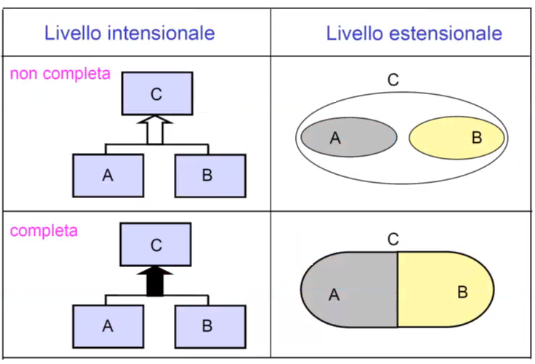
\includegraphics[scale=0.7]{generalizzazione.png}
        
        \label{<label>}
    \end{figure}
 Un ulteriore caratteristica della generazione è l’esclusività, una generalizzazione esclusiva prevede che un elemento possa appartenere solo a una delle categorie (uomo o donna). In caso vi siano più appartenenze, si definisce sovrapposto, ad esempio uomo donna e dottore (un’istanza può essere sia dottore che uomo o donna). 
    \\Come possiamo vedere, nella relazione  \textit{completa}, l'unione dei due sottoinsiemi A e B è proprio 
    l'insieme "padre" C. Nella relazione \textit{NON completa}, invece, ci saranno alcuni elementi di C che non fanno
    parte ne di A e ne di B.
    \\
    Una entità può avere \textbf{al massimo una e una sola} entità padre.

    \subsubsection{Principio di ereditarietà}
    Ogni proprietà del padre è anche una proprietà del figlio, che però non viene esplicitamente riportata nello schema concettuale.
    \\L'entità figlio può avere degli attributi in più rispetto all'entità padre.

    \newpage
    \subsection{Strategie di Progetto}
    Come procediamo con tante specifiche anche dettagliate?

    \begin{itemize}
        \item top-down
        \item bottom-up
        \item inside-out
    \end{itemize}

    \subsubsection*{Top-down}
    Si parte da uno schema iniziale molto astratto ma completo, che viene successivamente
    raffinato fino ad arrivare allo schema finale.\\Si parte dall'alto, e mano a mano si scende

    \subsubsection*{Bottom-up}
    Si suddividono le specifiche in modo da sviluppare semplici schemi parziali ma dettagliati,
    che poi vengono integrati tra di loro

    \subsubsection*{Inside-out}
    Parto dal primo termine e mano a mano sviluppo.
    \\\\
    Esiste anche una \textbf{strategia ibrida}, che è un insieme di tutte e 3.
    \begin{figure}[htbp]
        \centering
        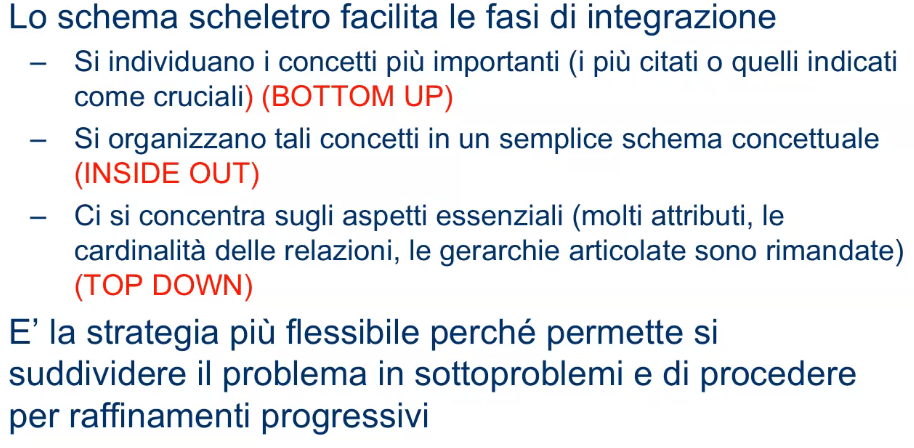
\includegraphics[scale=0.5]{ibrido.png}
        
    \end{figure}    

    \newpage
    \section{Modello Relazionale}
    Un modello dei dati è un insieme di concetti per organizzare i dati 
    e descriverne la struttura. Questo modello deve essere comprensibile a un elaboratore.
    La componente fondamendale di ogni modello sono i \textbf{meccanismi di strutturazione}.
    \\\\Il \textbf{Modello Relazionale} è il modello di dati più diffuso.
    \\\\Permette di definire per mezzo del costruttore relazione che permette di organizzare
    i dati in insiemi di record a struttura fissa. Una relazione è spesso rappresentata da una tabella.
    \textit{La relazione è un modo di relazionare i dati. Non è una relazione matematica ne è una relazione del modello ER.}

    \begin{figure}[htbp]
        \centering
        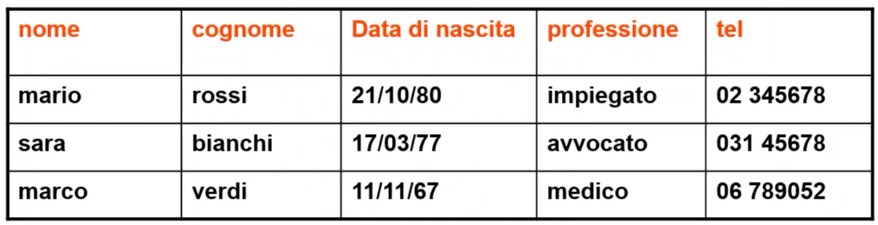
\includegraphics[scale=0.5]{rel.png}
    \end{figure}

    Il Livello Logico è \textbf{indipendente} da quello fisico: una tabella è usata nello stesso modo
    sia nel livello logico che nel livello fisico.
    \\\\
    In una relazione non ci sono più tuple con lo stesso valore. Altrimenti non sarebbe una relazione.

    \subsection*{Definizione di \textit{Schema di Relazione}}
    Un nome $R$ con un insieme di attributi $X = \{A_1, A_2, ..., A_n\}$\\
    es: STUDENTI(Matricola, Cognome, Nome, DataNascita)

    \subsection*{Definizione di \textit{Schema di Base di Dati}}
    Insieme di schemi di relazione con nomi diversi:
    \\R = {STUDENTI(...), ESAMI(...), CORSI(...)}
    \\R = \{$R_1(X_1), ..., R_n(X_n)$\}

    \newpage
    \subsection*{Definizione di \textit{Tupla}}
    Una tupla su un insieme di attributi X è una funzione \textit{t} che associa a ciascun attributo A in X
    un valore del dominio di A.
    \\t[A] oppure t.A denota il valore della tupla t sull'attributo A.


    \subsection*{Chiave}
    Insieme di attributi che identificano univocamente le tuple di una relazione.
    \\Formalmente:
    \begin{itemize}
        \item Un insieme K di attributi è \textbf{superchiave} per r se r non contiene
        due tuple distinte $t_1$ e $t_2$ tali che $t_1[K] = t_2[K]$.
        \item K è \textbf{chiave} per r se è una superchiave minimale per r
        \\(minimale significa che se si dovesse eliminare un attributo della superchiave, essa 
        non risulterebbe più una superchiave)
        \\
    \end{itemize}
    L'esistenza delle chiavi garantisce l'accessibilità a ciascun dato della base di dati.
    \newpage
    All'interno di una relazione, però, ci possono essere dei valori \textit{nulli}.
    \\Tre casi differenti: 
    \begin{itemize}
        \item Valore sconosciuto
        \item Valore inesistente
        \item Valore senza informazione
    \end{itemize}

    I DBMS non fanno distinzione tra questi casi.

    \subsection{Vincoli di integritrà}
    Alcuni esempi di vincoli di integrità:
    \begin{itemize}
        \item Valori nulli
        \item Valori fuori del dominio
        \item Tuple incosistenti 
        \item Tuple con valori uguale per chiavi
        \item Valori inesistenti in attributi usati per corrispondenze tra relazioni
    \end{itemize}
    I vincoli di integrità vengono usati per descrivere in modo più accurato la realtà dei fatti.
    Danno un contributo alla "qualità dei dati" e sono utili nella progettazione. 
    Sono anche usati dai DBMS nella esecuzione delle interrogazioni.
    \\\\Alcune volte, però, non tutte le proprietà di interesse sono rappresentabili per mezzo di vincoli 
    di integrità esprimibili direttamente. Verrano gestiti al di fuori della base di dati. 
    \newpage
    \subsubsection*{Tipi di vincoli}
    \begin{itemize}
        \item Vincoli su \textbf{valori} (un voto di esame non può andare oltre a 30)
        \item Vincoli di \textbf{tupla} (una lode può essere data solo a un voto di valore 30)
        \item Vincoli di \textbf{chiave} (non possono esistere due chiavi)
    \end{itemize}
    \begin{figure}[htbp]
        \centering
        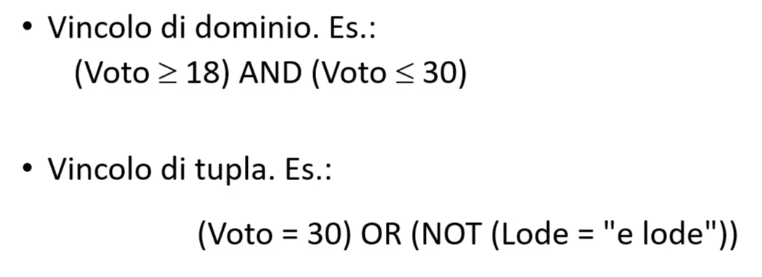
\includegraphics[scale=0.5]{vincoli.png}
        
    \end{figure}

    Esistono anche dei \textit{Vincoli \textbf{interrelazioni}} che coinvolgono più relazioni:
    \begin{itemize}
        \item Vincoli di integrità \textbf{referenziale}
    \end{itemize}

    \subsection{Vincoli di Integrità Referenziale}
    Un vincolo di integrità referenziale è un vincolo di integrità \textbf{interrelazionale}, ovvero si verifica quando andiamo
    a trattare due o più relazioni. 
    \\\\Una \textbf{Foreign Key} (vincolo di integrità referenziale) fra gli attributi X (uno o più attributi) di una relaizone $R_1$ e un'altra relazione $R_2$ impone ai valori 
    su X in $R_1$ di comparire \textbf{come valori della chiave primaria di $R_2$}.

    \begin{figure}[htbp]
        \centering
        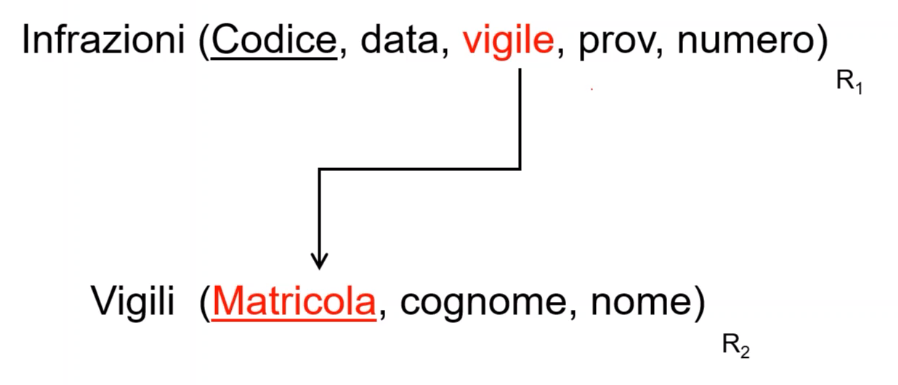
\includegraphics[scale=0.5]{foreignkey.png}
        \\\textit{Nel compitino \textbf{Le foreign key vanno cerchiate!!}}
    \end{figure}

    \section{Progettazione Logica}




    \section{SQL}
    Structured Query Language è un linguaggio dichiarativo per la definizione e la manipolazione dei dati in database 
    relazionali, adottato da molti DBMS.
    \\\\
    SQL è \textbf{relazionalmente completo}: ogni espressione dell'algebra relazionale
    può essere tradotta in SQL. Esso adotta la logica a 3 valori (T, F, U).
    \\Il modello dei dati di SQL è basato su \textbf{tabelle} anzichè \textbf{relazioni}.
    \\\\SQL contiene:
    \begin{itemize}
        \item DDL (Data Definition Language) - operazioni di definizione e modifica di schemi
        \item DML (Data Manipulation Language) - operazioni di inserimento, modifica e cancellazione di dati
    \end{itemize}

    \subsection*{Istruzioni Principali di DML}
    \begin{itemize}
        \item SELECT - Operazioni di interrogazione. Formula query come quelle dell'AR o richieste più elaborate.
        \item INSERT, DELETE, UPDATE - Operazioni di aggiornamento. Inserisce, elimina, aggiorna tuple.
    \end{itemize}

    \subsection*{Istruzioni Principali di DML}
    \begin{itemize}
        \item CREATE SCHEMA - Crea un nuovo schema
        \begin{figure}[htbp]
            \centering
            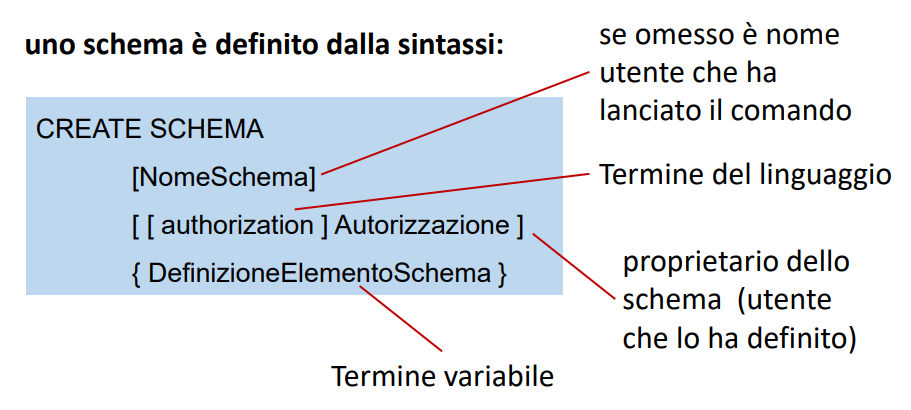
\includegraphics[scale=0.5]{createschema.png}
        \end{figure}
        \item CREATE TABLE - Crea una nuova tabella;
        \\Una tabella è costituita da una collezione ordinata di attributi e da
        un insieme (eventualmente vuoto) di vincoli.
        \begin{figure}[htbp]
            \centering
            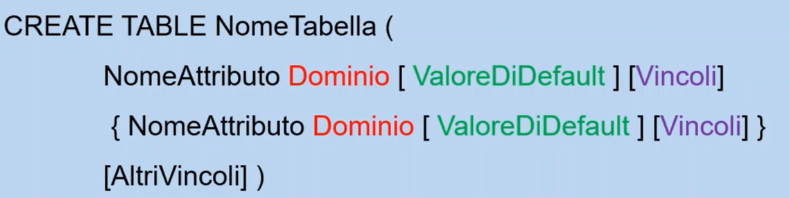
\includegraphics[scale=0.5]{createtable.png}
        \end{figure}
    \end{itemize}

    \subsection*{Domini Elementari}
    SQL ha 6 domini predefiniti
    \begin{itemize}
        \item Carattere (VARCHAR, CHAR)
        \item Numerico Esatto (INTEGER)
        \item Numerico Approssimato
        \item Data/Ora (TIMESTAMP, DATE, TIME)
        \item Intervallo Temporale
        \item Boolenan (ex Bit)
    \end{itemize}
    C'è anche la possibilità di definire nuovi domini usando \textbf{CREATE DOMAIN}.
    \begin{figure}[htbp]
        \centering
        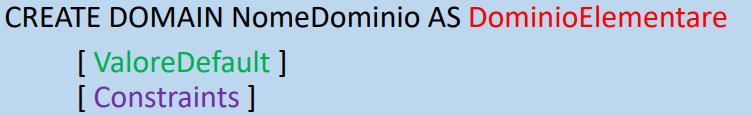
\includegraphics[scale=0.5]{createdomain.png}
    \end{figure} 
    \\Questo comando definisce un nuovo dominio elementare utilizzabile in definizioni di relazioni.
    \begin{figure}[htbp]
        \centering
        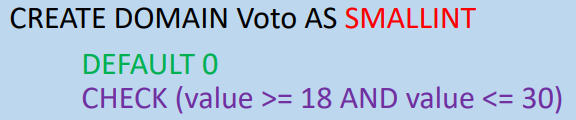
\includegraphics[scale=0.5]{createvoto2.png}
    \end{figure}

    \subsection*{Vincoli}
    Un vincolo è una regola che specifica delle condizioni sui valori di un elemento
    dello schema del database.
    \\\\Un vincolo può essere associato ad una tabella, attributo o dominio.

    \begin{itemize}
        \item Vincoli Intrarelazionali - proprietà sempre valida all'interno di una relaizone
        \begin{itemize}
            \item NOT NULL - il valore deve essere non nullo
            \item UNIQUE - i valori devono essere non ripetuti
            \item PRIMARY KEY - chiave primaria della tabella
            \item CHECK - definisce condizioni complesse
        \end{itemize}
        \item Vincoli Interrelazionali - proprietà sempre valida tra relazioni diverse
        \item \begin{itemize}
            \item FOREIGN KEY, REFERENCES - permettono di definire le chiavi esterne.\\
            Impone ai valori degli attributi X nella tabella Figlio di comparire \textit{come valori della chiave primaria della tabella Padre}
            \item CHECK
        \end{itemize}
    \end{itemize}
    Se viene eseguita una operazione di aggiornamento che porta alla
    violazione di un vincolo di integrità referenziale, (per ogni vincolo
    visto) lo stato della base di dati diventa non valido.Sono perciò definite un insieme di politiche per evitare che questo
    accada. Tali politiche vanno dichiarate nella dichiarazione DDL dello
    schema.
    \begin{itemize}
        \item CASCADE - l'operazione di modifica/cancellazione viene propagata alla tabella interna
        \item SET NULL - NULL nella tabella figlio in entrambi i casi
        \item SE DEFAULT - default nella tabella figlio in entrambi i casi
        \item NO ACTION - rifiutata in entrambi i casi
    \end{itemize}

    \newpage
    \subsection{Interrogazioni SQL}
    Le interrogazioni di SQL avvengono tramite l'istruzione \textbf{SELECT} (che non significa "seleziona").
    \begin{figure}[htbp]
        \centering
        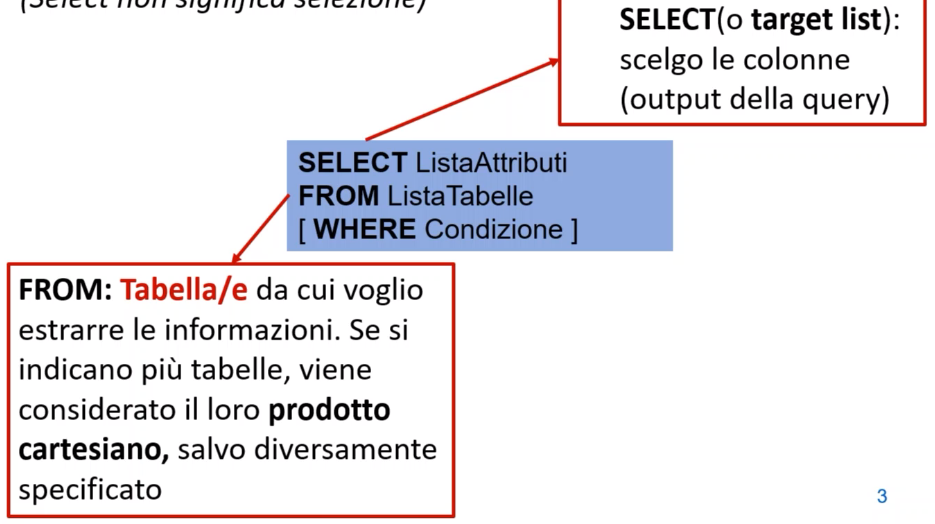
\includegraphics[scale=0.5]{select.png}
    \end{figure}
        



    
    
    \end{document}